\documentclass{article}
\usepackage{graphicx} % Required for inserting images
\usepackage{amsmath}
\usepackage{amsfonts}
\DeclareMathOperator*{\argmax}{arg\,max}
\DeclareMathOperator*{\argmin}{arg\,min}

\usepackage{tikz}

\newcommand*{\xMin}{0}%
\newcommand*{\xMax}{4}%
\newcommand*{\yMin}{0}%
\newcommand*{\yMax}{4}%

\usetikzlibrary{positioning}% for specifications like "left=of ..."
\usetikzlibrary{automata}% automata related stuff
\usetikzlibrary{calc}% for calculating coordinates, like ($...$)
\usetikzlibrary{arrows.meta}% arrow head Stealth[round]

% define settings common to several automata
\tikzset{FAstyle/.style={
    shorten >=1pt,% leave a thin space between arrow head and target node
    node distance=3cm,% grid size
    on grid,% arrange nodes on a grid
    auto,% automatic placements of labels
    every state/.style={% define appearance of nodes
      draw=blue!50,
      very thick,
      top color=white,
      bottom color=blue!20,
      minimum size=0pt
    },
    >=Stealth[round],
    thick,
    draw=black!50
  }
}

\title{DS 598 HW1}
\author{Write your name here}

\begin{document}

\maketitle

\paragraph{Instructions:} Please write your solution in latex and submit the compiled PDF to the blackboard submission portal. You can use the latex source file for each HW assignment as a starting point.

\paragraph{Problem 1.} Calculate the $V^*$ function for the following MDP. Each grid represent a state and there are 4 actions in each state traveling to the 4 adjacent states respectively. Numbers in the grid represent reward for getting into the grid. Let $\gamma=0.9$ be the discounting factor.


\begin{figure}[!h]
\centering
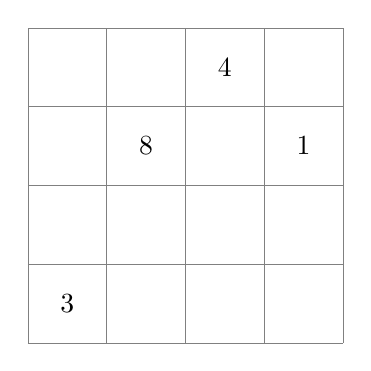
\begin{tikzpicture}
    \foreach \i in {\xMin,...,\xMax} {
        \draw [very thin,gray] (\i,\yMin) -- (\i,\yMax);
    }
    \foreach \i in {\yMin,...,\yMax} {
        \draw [very thin,gray] (\xMin,\i) -- (\xMax,\i);
    }
    \node at (0.5,0.5) {3};
    \node at (3.5,2.5) {1};
    \node at (2.5,+3.5) {4};
    \node at (1.5,+2.5) {8};
\end{tikzpicture}
\caption{Problem 1 MDP.}
\end{figure}

\paragraph{Problem 2.} During the lecture, we derived the Bellman Equation (BE) for $V^\pi$ and Bellman Optimality Equation (BOE) for $V^*$. Derive the Bellman equation for $Q^\pi$ and $Q^*$. You can use the BE and BOE for $V$ functions as a starting point.

\paragraph{Problem 3.} In the lecture we've proved that $V^* = V^{\pi^*}$, where $\pi^*$ is defined as
\begin{align*}
    \pi^*(s) = \argmax_{a} \left[r(s,a) + \gamma \mathbb{E}_{s'\sim P(\cdot|s,a)}V^*(s')\right]
\end{align*}
Prove that $Q^* = Q^{\pi^*}$. You can use the established equality for $V$ as a starting point.

\paragraph{Problem 4.} Prove that the Value Iteration (VI) algorithm converges, i.e. show that the Bellman Optimality Equation satisfies the contraction property.

\paragraph{Problem 5.} Calculate the occupancy measure $d^\pi_\mu$ for the following MDP: There are 4 states $S_1,S_2,S_3,S_4$. $\mu$ is a point-mass on $S_1$, i.e $\mu(S_1)=1$ and $\mu(S_2)=\mu(S_3)=\mu(S_4)=0$. The transition probability following $\pi$ is indicated by the arrow and numbers in the plot. The discounting factor is set to $\gamma=0.9$.

\begin{figure}[!h]
\centering
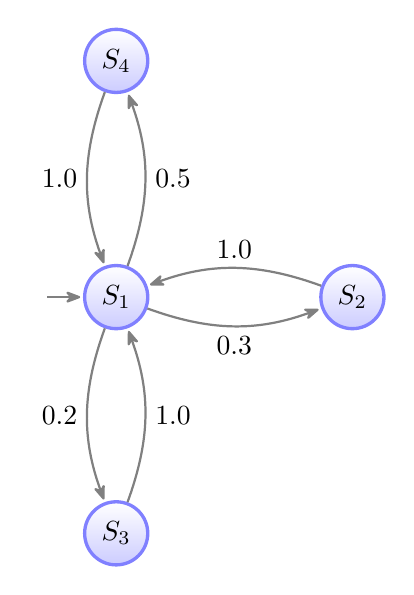
\begin{tikzpicture}[FAstyle]
  \node[state,initial,initial text=] (1) {$S_1$};
  \node[state,right=of 1] (2) {$S_2$};
  \node[state,below=of 1] (3) {$S_3$};
  \node[state,above=of 1] (4) {$S_4$};
  \path[->] (3) edge[bend right=20] node[swap]{1.0} (1)
            (1) edge[bend right=20] node[swap]{0.2} (3)
            (4) edge[bend right=20] node[swap]{1.0} (1)
            (1) edge[bend right=20] node[swap]{0.5} (4)
            (2) edge[bend right=20] node[swap]{1.0} (1)
            (1) edge[bend right=20] node[swap]{0.3} (2)
  ;
\end{tikzpicture}
\caption{Problem 5 MDP.}
\end{figure}
\end{document}

